\section{On-demand open-world evaluation}
\label{sec:method}

Pooling bias is essentially a sampling bias problem where relational tuples from pooled systems are overrepresented and those from new systems are underrepresented in the evaluation dataset.
We could of course completely eliminate the bias by exhaustively annotating the entire document corpus, but that would be a laborious and prohibitively expensive task:
  using the interfaces we've developed (described in detail in \refsec{evaluation}), it costs about \$20 to annotate a single document by non-expert crowdworkers, leading to an estimated cost of at least \$200,000 for a reasonably large corpus of 10,000 documents.
The annotation effort would cost significantly more with expert annotators.
% TODO: highlight contrast with pooling.

In constrast, we propose a new paradigm called on-demand open-world evaluation which takes a lazy approach to dataset construction by annotating predictions from systems \textit{only when they are underrepresented}, thus correcting for pooling bias as it arises.
In this section, we'll formalize the problem solved by on-demand open world evaluation independent of KBP and describe our solution that allows us to accurately estimate evaluation metrics without bias in a cost-effective manner. 
We'll then instantiate the framework for KBP in \refsec{application}.

\subsection{Problem statement}
Let $\sX$ be a universe of possible system outputs (e.g.\ relational tuples),
  $\sY \subseteq \sX$ be an unknown subset of this universe corresponding to the correct elements in $\sX$,
  $X_1, \ldots X_m \subseteq \sX$ be known subsets that correspond to the predicted output from $m$ systems,
  and let $Y_1, \ldots, Y_m$ be the intersection of $X_1, \ldots, X_m$ with $\sY$.
Our goal is estimate the precision, $\pi_i$, and recall, $\rho_i$, of the set of predictions $X_i$ to within a certain confidence interval $\epsilon$.
Formally, let $f(x) \eqdef \I[x \in \sY]$ and $g_i(x) = \I[x \in X_i]$, then:
\begin{align*}
  \pi_i  &\eqdef \E_{x \sim X_i}[f(x)] &
  \rho_i &\eqdef \E_{x \sim \sY}[g_i(x)],
\end{align*}
where $x$ is sampled from $X_i$ and $\sY$ according to distributions $p_i(x)$ and $p'(x)$ respectively.
We assume that $p_i(x)$ is known, e.g.\ the uniform distribution over $X_i$, and that samples from $p'(x)$ can be obtained, even if it is unknown.

In on-demand open-world evaluation, we are allowed to ask if $x \in \sY$ (e.g.\ by assessing a system's prediction) or for samples from $\sY$ (e.g.\ by exhaustively annotating a document) at a certain (monetary) cost.
Typically, checking if $x \in \sY$ can be significantly cheaper than asking for samples from $\sY$.

Clearly, $\pi_i$ and $\rho_i$ can both be estimated by sampling from $X_i$ and $\sY$ respectively:
\begin{align*}
  \pih_i^{(s)} &= \sum_{x \in \Xh_i} f(x) & \rhoh_i^{(s)} &= \sum_{x \in \Yh_0} g_i(x).
\end{align*}
However, simple statistics tell us that we could require at least 10,000 samples each to estimate $\pi$ and $\rho$ to $\pm 1\%$, which would be quite costly on a per-system basis.
To make the system practically viable, we'd like be able to reuse the samples we've collected and only spend money to annotate data when absolutely necessary.
In the rest of this section, we'll see how to do this by answering the following three key questions:
\begin{enumerate}
  \item Suppose we have evaluated $f(x)$ on samples $\Xh_1, \ldots, \Xh_m$ from $X_1, \ldots, X_m$ respectively. How should we best use all of these samples when estimating $\pi_i$?
  \item 
    Can we use the samples $\Xh_1, \ldots, \Xh_m$ when estimating $\rho_i$ in conjunction with samples $\Yh_0$ from $\sY$?
  \item Finally, in practice, we only see the sets $X_1, \ldots, X_m$ sequentially, as and when they are submitted to the evaluation platform. How many samples should we draw from $X_m$, given existing samples $\Yh_0$ and $\Xh_1, \ldots, \Xh_{m-1}$?
\end{enumerate}

\subsection{Amortizing costs when estimating precision}

Intuitively, if a set $X_j$ has a significant overlap with $X_i$, we expect that we should be able to its samples when estimating $\pi_i$.
However, it might be case that $X_j$ overlaps with $X_i$ only when $p_i(x)$ is relatively small, in which case the sample $\Xh_j$ is not representative of $X_i$ and a naive combination could lead to the wrong estimate of $\pi_i$.
We address this problem by using importance sampling \citep{owen2013monte}.

In particular, the estimator that we propose is:
\begin{align*}
  \pih_i &= \sum_{j=1}^m \frac{w_{ij}}{n_{j}} \sum_{x \in \Xh_j \intersection X_i} \frac{p_i(x) f(x)}{q_i(x)},
\end{align*}
where $n_{j} = |X_j|$, $q_i(x) = \sum_{j=1}^m w_{ij} p_j(x)$ and $w_{ij} \ge 0$ are mixture parameters such that $\sum_{j=1}^m w_{ij} = 1$ and $q_i(x) > 0$ wherever $p_i(x) > 0$.
This last condition is easy to guarantee by setting $w_{ii} > 0$.

In \appendixref{sampling} we prove that $\pih_i$ is an unbiased estimator of $\pi_i$ and also work out an expression for its variance. 
The variance of course depends on $f(x)$, but the general intuition is that 
$\pih_i$ will have high variance if $q_i(x) \ll p_i(x)$.
This motivates the choice $w_{ij} \propto n_{j} \sum_{x \in \sX} p_j(x) p_i(x)$, which assigns $0$ weight to any set $X_j$ that has no overlap with $X_i$ and also has the optimal choice of weights if all the sets are identical, i.e.\ $p_j = p_i$ for all $j$.

% TODO: Figure that compares our scheme with equivalent of pooling.
\fake{On simulated experiments on the TAC-KBP dataset, we find a 4-fold decrease in variance using the proposed $\pih$ 
when compared to estimating $\pi_i$ solely using $\Xh_i$}.

\subsection{Amortizing costs when estimating recall}
When estimating recall, we ideally would like to compare the performance of the system on samples drawn from $\sY$.
Unfortunately, in practice, it is typically much harder to sample $\sY$ than it is to evaluate $f(x)$, because the former needs us to exhaustively annotate a document.
In contrast, it is very easy to compare a system's recall relative to \textit{other} systems by using the samples $\Xh_i$ we've already collected.
This mode of computing recall, called pooled recall, can be biased and typically overestimates recall on the universe of relations.
However, we know that if a system represents only a fraction $\nu_i$ of the pool of all systems and that the pool represents a fraction $\theta$ of $\sY$, $\rho_i$ must equal $\theta \nu_i$.

%However, the recall of the system $\rho_i$, pooled recall $\nu_i$ and the recall of the pool $\theta$ share a simple relationship.
%estimate the recall of a system $i$ relative to all the pool of all other submitted systems.
%We exploit the fact that the recall of a system $i$, $\rho_i$ can also be expressed as the recall of the system \textit{relative} to the pool, $\nu_i$ and the recall of the pool itself $\theta$: $\rho_i = \theta \nu_i$.

With this in mind, we use a smaller sample $\Yh_0$ from $\sY$ to estimate $\theta$ and then use the rest of $\Xh$ to estimate $\nu_i$.
In \appendixref{sampling} we show that the final estimator, $\rhoh_i \eqdef \thetah \nuh_i$, is unbiased and has a variance of,
\begin{align*}
  \sigma^2_\rho &= \theta \sigma^2_\nu + \nu_i \sigma^2_\theta + \sigma^2_\nu \sigma^2_\theta.
\end{align*}
With sufficient samples, $\sigma^2_\nu$ can be made quite small, so that the leading term in the variance is $\nu_i \sigma^2_\theta$ and because typically $\nu_i \ll 1$, we expect the variance of our proposed estimator to be less than that of the estimator constructed by using $\Yh_0$ alone.

% TODO: figure
\fake{On simulated experiments on the TAC-KBP dataset, we find a 2-fold decrease in variance using the proposed estimator $\rhoh$ 
when compared to estimating $\rho_i$ solely using $\Yh_0$}.

\subsection{Adaptively drawing samples for new sets}
Finally, the desired property for our framework is to annotate new data only when necessary, i.e.\ a new submission $X_m$ contains sufficiently diverse output.
We formalize this statement by requesting for a target variance $\epsilon$.
The variance of $\pih_m$ is a complex non-convex function, but we know that it is monotonically decreasing in $n_m$, the number of samples drawn from the new output, $X_m$.
Consequently it is quite easy to solve for the number of samples needed to achieve a target variance of $\epsilon$ using a bisection method.
% TODO: figure
\fake{Simulated experiment of how many samples are required}.

\begin{algorithm}
  \caption{\label{alg:on-demand-sampling} The on-demand open-world evaluation methodology}
\begin{algorithmic}
  \REQUIRE{
  A sequence of predicted output sets $X_1, \ldots X_m \subseteq \sX$,
  a method of evaluating $f(x) = \I[x \in \sY]$ and a method of sampling $x \sim \sY$,
  desired confidence intervals $\epsilon_\pi$ and $\epsilon_\rho$.
  }
  \ENSURE{Unbiased predictions of precision, $\pih_1, \ldots, \pih_m$ and recall $\rhoh_1, \ldots \rhoh_m$.}

  % Collect a dataset Y_0
  \STATE{Sample a set $\Yh_0$ from $\sY$ based on $\epsilon_\rho$.}
  % For each sample X_i, 
  \FOR{$i = 0$ \TO{} $i = m$}
  % compute the optimal number of samples $n_i$ required to estimate $\pih_i$ to within $\epsilon$ given $\Xh_{1} - \Xh_{i-1}.
  \STATE{Compute the minimum number of samples $n_i$ required to estimate $\pi_i$ within $\epsilon_\pi$.}
  % Draw $n_i$ samples from $X_i$ and evaluate $f(x)$ on these samples.
  \STATE{Evaluate $f(x)$ on $n_i$ samples drawn from $X_i$.}

  \FOR{$j = 0$ \TO{} $j = i$}
    % For j,
    % Use $\Xh_1 ... \Xh_m$ to evaluate or update $\pih_j$.
    % Use $\Xh_1 ... \Xh_m$ to evaluate or update $\rhoh_j$.
    \STATE{Use $\Xh_1, \ldots \Xh_i$ to update estimates for $\pi_j$ and $\rho_j$.}
  \ENDFOR{}
  \ENDFOR{}
\end{algorithmic}
\end{algorithm}

\refalg{on-demand-sampling} summarizes the whole approach. 
%TODO: a summary/outline diagram.

%\begin{figure}[t]
%  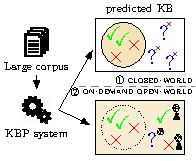
\includegraphics[width=\columnwidth]{figures/overview}
%  \caption{\label{fig:overview}
%  In knowledge base population (KBP), systems construct a knowledge base (KB) containing \textit{relations}. % about \textit{entities} 
%  %such as where a person was born or who a company's founder is, 
%  from a large document corpus.
%  \encircle{1}
%  In closed-world evaluation, %only relations that intersect with an existing set of annotated facts
%  %, usually constructed from other output of other systems,
%  all relations ouside an annotated set are incorrectly assumed to be negative.
%  %are considered to be true and all others are assumed false.
%  %This can significantly penalize a novel system that predicts new facts outside what has already been annotated.
%  \encircle{2}
%  In on-demand open-world evaluation,
%  predicted relations are sampled and immediately evaluated through crowdsourcing
%  to provide an unbiased estimate of open-world performance. % in an open-world setting.
%  \todo{fix figure}.
%  }
%\end{figure}
%
